\documentclass[12pt,a4paper,openright,twoside]{book}
\usepackage[utf8]{inputenc}
\usepackage{disi-thesis}
\usepackage{code-lstlistings}
\usepackage{notes}
\usepackage{shortcuts}
\usepackage{acronym}

\school{\unibo}
\programme{Corso di Laurea Magistrale in Ingegneria e Scienze Informatiche}
\title{Development Process of a Compiler Plugin for Aggregate Computing}
\author{Francesco Magnani}
\date{\today}
\subject{Software Process Engineering}
\supervisor{Danilo Pianini}
\cosupervisor{Nicolas Farabegoli}
\morecosupervisor{Angela Cortecchia}
\session{III}
\academicyear{2023-2024}

% Definition of acronyms
\acrodef{IoT}{Internet of Thing}
\acrodef{vm}[VM]{Virtual Machine}
\acrodef{IDE}[IDE]{Integrated Development Environment}
\acrodef{CI}[CI]{Continuous Integration}
\acrodef{AST}[AST]{Abstract Syntax Tree}
\acrodef{KAPT}{Kotlin Annotation Processing Tool}
\acrodef{KSP}{Kotlin Symbol Processing}
\acrodef{IR}{Intermediate Representation}
\acrodef{DSL}{Domain Specific Language}
\acrodef{IR}{Intermediate Representation}
\acrodef{FIR}{Frontend Intermediate Representation}
\acrodef{PSI}{Programming Structure Interface}


\mainlinespacing{1.241} % line spacing in mainmatter, comment to default (1)

\begin{document}

\frontmatter\frontispiece

\begin{abstract}	
Max 2000 characters, strict.
\end{abstract}

\begin{dedication} % this is optional
Optional. Max a few lines.
\end{dedication}

%----------------------------------------------------------------------------------------
\tableofcontents   
\listoffigures     % (optional) comment if empty
\lstlistoflistings % (optional) comment if empty
%----------------------------------------------------------------------------------------

\mainmatter

%----------------------------------------------------------------------------------------
\chapter{Introduction}
\label{chap:introduction}
%----------------------------------------------------------------------------------------

Analyzing characteristics of the source code without necessarily building and
executing it (i.e., static analysis) is a process that has been studied and
implemented in various forms during the last decades. Various tools have been
developed to perform such a task, each with its own strengths and weaknesses.
%
The need for such a tool is often evident in the software development process,
where ensuring the \textbf{quality} and \textbf{robustness} of software systems
is a critical concern. Using code quality analysis techniques is also a powerful
mean to avoid situations of ``technical debt''
\cite{DBLP:conf/sigsoft/ErnstBONG15}, that targets the system quality in
maintenance and evolution.

As the system grows in complexity, so does the variety of errors and
vulnerabilities that can be detected through tools (e.g., concurrency management
issues, error handling, etc.). At the same time, adhering to coding standards
helps to avoid both trivial and non-trivial errors from the outset.
Additionally, these are among the easiest types of tools to integrate, often
already included within \acp{IDE}.
%
The effectiveness of static analysis tools has been the subject of various
studies,  \cite{DBLP:journals/jss/LenarduzziPSLP23} evaluating their detection
capabilities, agreement, and precision. Some of these studies revealed a low
degree of agreement among the tools and highlighted the need for a better
understanding of their actual capabilities. More advance tools have been used
also to rewrite code and help with the development of very complex systems,
like \emph{Coccinelle} for the Linux kernel
\cite{DBLP:conf/eurosys/PadioleauLHM08}\cite{DBLP:conf/usenix/LawallM18}.
%
More over, in the last years, the static analysis tools have become more popular
and easier to use, becoming protagonists of many \ac{CI} pipelines
\cite{DBLP:conf/msr/ZampettiSOCP17} that automatically performs checks on the
entire source code, embracing change and evolution of the software without
making it a threat \cite{DBLP:books/daglib/0015650}, backed by a solid safety
net.

If looked from another perspective, automated static analysis tools and
compilers share significant similarities in their operations. Both perform
thorough examinations of source code without executing it, aiming to identify
errors, enforce coding standards, and optimize performance. Most of what
compilers do on the static analysis side is to facilitate code optimization and
error detection during the compilation process. In fact, a compiler can be
viewed as a form of static analysis tool, as it analyzes code to generate
executable programs and associated debugging information
\cite{DBLP:journals/queue/Thomson21}.
%
Specialized static analysis tools, on the other hand, extend beyond the
capabilities of standard compilers by offering additional functionalities and
broader diagnostic capabilities. They offer a broader range of diagnostic rules,
enabling the detection of specific and uncommon bugs that compilers might
overlook.
%
What if, however, the compiler were extended beyond its core functionality,
incorporating specialized capabilities that go beyond the scope of a
general-purpose environment? These extensions could be designed to address the
unique requirements of a specific project or domain. This is precisely where
\textbf{compiler plugins} come into play.

\section{Definition and Purpose of Compiler Plugins}

Compiler plugins are dynamic modules that interact with the compiler during its
various phases, enabling the introduction of new functionalities or the
modification of existing behaviors. They serve as intermediaries that can
inspect, modify, or enhance the compilation process, providing developers with
the flexibility to implement domain-specific checks, optimizations, or
transformations, all without altering the compiler's core architecture. 
%
For instance, in the context of the GNU Compiler Collection
(GCC), plugins allow for the addition of new features without necessitating
modifications to the compiler itself (mostly, again, for optimization purposes).

\subsection{Types of Compiler Plugins}

Compiler plugins can be broadly categorized based on the phase of compilation they target:

\begin{itemize}
  \item \textbf{Frontend Plugins}: These plugins operate during the initial
  stages of compilation, focusing on tasks such as syntax analysis, semantic
  analysis, and \ac{IR} generation. They are useful also for
  implementing custom syntax extensions, enforcing coding standards, or
  performing static code analyzes. For example, in the \emph{Rust} programming
  language, compiler plugins can introduce new syntax extensions and lint
  checks. 

  \item \textbf{Backend Plugins}: Functioning in the latter stages of
  compilation, backend plugins are concerned with code optimization, machine
  code generation, and platform-specific adjustments. They can be utilized to
  implement custom optimizations, support additional hardware
  architectures and more.
\end{itemize}

\subsection{Compiler Plugins in Kotlin}

Kotlin, a statically typed programming language developed by JetBrains, offers
robust support for compiler plugins, allowing developers to highly customize the
compilation process to their specific needs. 
%
Kotlin's compiler architecture facilitates the creation of plugins that can
modify or extend its behavior during compilation. For example, the
\emph{all-open} compiler plugin in Kotlin allows classes annotated with a
specific annotation to be open without the explicit \lstinline{open} keyword,
adapting Kotlin to the requirements of frameworks that need classes to be
open. 

When guiding developers towards the creation of compiler plugins, JetBrains
compares them to \textbf{Annotation Processors}
\cite{JetBrains:KotlinCompilerPlugin}. Annotation processors are a powerful
feature in many modern programming languages, including Java and Kotlin, that
allow developers to generate code, validate code, and perform various
compile-time checks based on \textbf{annotations} present in the source code.
%
In Java, annotation processors are part of the Java Compiler API and can be used
to generate additional source files, validate the correctness of the code, and
even modify the \ac{AST} of the code being compiled. They are
commonly used in frameworks and libraries to reduce boilerplate code and enforce
coding standards.
%
Kotlin also supports annotation processors through the \ac{KAPT} — which is, in
fact, a compiler plugin itself — that allows Kotlin code to interoperate with
Java annotation processors and, more recently, the \ac{KSP}, another compiler
plugin introduced as ``an API that you can use to develop lightweight compiler
plugins''. The former enables developers to leverage existing Java annotation
processors in their Kotlin projects and the latter, on the other hand, provides
a more efficient and Kotlin-specific way to generate code at compile time,
offering a new approach that is much more integrated with Kotlin symbols.

\subsection{Compiler Plugins advantages}

Compiler plugins and Annotation Processors, however, have some very distinct
functionalities. While Annotation Processors are limited to generating source
code and performing checks based on annotations, compiler plugins can exploit a
very powerful API that can create and modify byte-code, elements inside the
\ac{IR} and more, allowing the developers to solve a whole new class of
meta-programming problems. Of course, Annotation Processors are typically easier
to write and maintain than compiler plugins, but this extra cost can be worth in
several cases, for example in the scenario that will be presented in this
thesis.

\section{Development of a Frontend Compiler Plugins}

At the time of writing, the development of frontend compiler plugins in Kotlin is
still a relatively less explored area compared to the backend ones. Because of the 
very little documentation and examples available, the development of frontend 
compiler plugins can be a challenging task, that quite often requires inspecting 
the Kotlin compiler source code to understand how to interact with it.
%
Frontend compiler plugins can be implemented using \textit{Extensions} to the
Kotlin compiler, a topic that will be covered more in detail in the following
chapters. This thesis presents the development process of a frontend compiler
plugin designed to build upon an existing \textit{backend} plugin. The primary
purpose of this frontend plugin is to perform static checks on source code,
ensuring compliance with specific rules related to the functionality of the
pre-existing backend plugin.

\subsection{The importance of Build Tools}

Before proceeding with the explanation of the main structure of this thesis, it
is important to mention the role of build tools in the development process of a
compiler plugin. Without a seamless integration of the compiler plugin during
the compilation process (and, as it will be shown, the testing process as well), the
development of a compiler plugin would be cumbersome and error-prone. 
%
Needless to say, a well-configured build tool is a fundamental requirement in
this context. Within the Kotlin ecosystem — on which this work focuses — the most
widely used build tool is \emph{Gradle}, and it will serve as the foundation for
the implementations discussed in this thesis.

\paragraph{Structure of the Thesis}

This thesis follows the development process of a frontend compiler plugin from
its initial steps, addressing the key challenges encountered as well as the
solutions proposed during the research and implementation phases. The next
chapter, \cref{chap:background}, provides an overview of the ongoing project for
which this frontend plugin is being developed, alongside the technical
background necessary to understand how a plugin can interact with the Kotlin
compiler.
%
\Cref{chap:contribution} delves into the core development process of the plugin,
discussing the design decisions, alternative approaches considered, and the
final implementation of the proposed \textbf{checkers}. Subsequently,
\cref{chap:evaluation} evaluates the plugin’s behavior, with a particular focus
on the testing methodology adopted, including the integration of a custom
testing framework named \emph{Subjekt}, developed specifically for this purpose.
%
Lastly, \cref{chap:conclusion} summarizes the primary contributions of this
thesis and outlines potential directions for future work, building on the
results and insights gained throughout this research.

%----------------------------------------------------------------------------------------
\chapter{Background: the Collektive case}
\label{chap:background}
%----------------------------------------------------------------------------------------

As already stated, the development of the frontend compiler plugin presented in
this thesis will be built on top of an existing backend plugin. The backend
plugin is part of a larger project named \emph{Collektive}, a Kotlin
multiplatform framework that provides a \ac{DSL} for the \textbf{Aggregate
Computing} \cite{Beal2015} paradigm. This chapter will provide an overview of
the concepts behind Collektive as well as the feature behind its backend plugin
and Kotlin compiler plugins development in general.

\section{Aggregate Computing}

The Aggregate computing paradigm is a novel approach to ``design, create and
maintain'' \cite{Beal2015} complex distributed systems, particularly in the 
context of the Internet of Things (IoT). The paradigm shifts the focus from
individual devices to regions of devices, abstracting away the details of their
number, position, and behavior. This abstraction enables developers to reason
about distributed systems in terms of \emph{collective} operations over spatial and
temporal fields, rather than device-to-device interactions. 

The foundation of aggregate programming is built on \textbf{field calculus}
\cite{Beal2014TowardsAU}, a set of constructs designed for spatial computing.
These constructs enable the implementation of robust coordination mechanisms,
such as self-stabilizing and scalable operations \cite{Viroli2018}
\cite{DBLP:journals/jlap/ViroliBDACP19}, which adapt dynamically to changes in
the environment. Applications of aggregate programming are particularly
impactful in large-scale scenarios, such as crowd management during public
events, where distributed devices coordinate to provide services like crowd
density estimation, dispersal advice, and navigation support.

Aggregate computing formalism has been proposed in various ways, introducing
syntaxes and semantics to support distributed, collective behaviors in dynamic
systems. Field calculus, as a foundational model, supports aggregate computing
by enabling global-level manipulation of computational fields through a
minimalistic syntax. 
%
Tools like Protelis \cite{DBLP:conf/saso/PianiniBV17}, ScaFi
\cite{DBLP:conf/ecoop/CasadeiV16} and the recently proposed eXchange Calculus
(XC) \cite{DBLP:journals/jss/AudritoCDSV24} extend field calculus principles,
providing programming frameworks and language constructs to bridge the gap
between theoretical models and practical implementations.

Managing the programming line of action for these kinds of systems is not
trivial, but several approaches have already been proposed, including static and
dynamic checks that can spot subtle bugs and vulnerabilities in the code, by
focusing on concepts like \textbf{neighborhood interactions} and \textbf{domain
alignment} \cite{DBLP:conf/saso/AudritoDVC16}.

\subsection{Main aspects}

In Aggregate Computing, the main model of the system consists of a \emph{network of 
intercommunicating devices}, which can be \emph{close} to one another therefore 
introducing a concept of \textbf{neighborhood}. 
%
Each device is equipped with sensors and actuators, enabling interaction with an
environment, and can communicate with other devices through a
\emph{message-passing} system. 

A key aspect of Aggregate Computing regards the execution model, which is based
on a local program identical for all devices. The system is governed by a
continuously executed loop that makes the devices \emph{receive messages},
\emph{produce a result through their internal behavior} and finally \emph{send
values to neighbors}. 
%
This simple structure allows for system to show self-organizing behaviors
emerging from the \emph{collective} of devices, and contemplates even complex
interactions of the devices with the environment (e.g. creation of new devices).

Finally, as already said, the \emph{field calculus} model can be implemented
through an ad-hoc API and syntax to perform operations on a \emph{computational
field} (i.e., a mapping from device locations to values in our example)
manipulating it over time, defining interactions between devices and finally
creating the emergent behavior.
%
After the previous tools already cited, it is now necessary to
introduce the Aggregate Computing framework that will be the target of the
frontend plugin in this thesis: \emph{Collektive}.

\section{Collektive: an Aggregate Computing Framework}

\emph{Collektive} is a modern Aggregate Computing framework developed in Kotlin 
that allows developers to easily write Aggregate Computing programs through a 
flexible \emph{internal} DSL. The framework is designed to be multiplatform,
targeting both JVM and JavaScript platforms, as well as native ones. 
%
Compared to some other existing Aggregate Computing frameworks, Collektive
offers a modern and idiomatic approach to writing Aggregate Computing programs,
with a static type system (as it is internal to Kotlin) and few, expressive
constructs like \lstinline{neighboring} and \lstinline{exchange}, which can be
used to implement a broad variety of interactions between devices (and also
Aggregate Computing patterns).

The project is organized in modules, with the main one being the \lstinline{dsl}
and \lstinline{compiler-plugin}, and is tested using the Alchemist simulator
\cite{DBLP:journals/jos/PianiniMV13}. 

\subsection{Collektive DSL: main concepts}

In order to understand how to work on Collektive programs, we first need to
understand its main usage. Collektive DSL is centered around the
\lstinline{aggregate} function, which is the entry point for the Aggregate
Computing program. The function uses a local ID to identify the device on which
is executed on and then accepts a function type with receiver
\lstinline{compute: Aggregate<ID>.() -> R} that performs the aggregate
computation using the \lstinline{Aggregate} interface members.
%
The \lstinline{Aggregate} interface provides several functions that represent
the main constructs of Collektive's implementation of the Aggregate Computing
paradigm. The most important ones are:
\begin{itemize}
  \item \lstinline{neighboring}: a function that observes expressions on
  neighbors, returning the related field;
  \item \lstinline{exchange}: a function that, taken from the documentation of
  Collektive, ``manages the computation of values between neighbors in a
  specific context''. In practice, it can be used to compute a new field of 
  values starting from initial values of neighbors;
  \item \lstinline{evolve}: updates an initial value iteratively computing an
  expression at each device;
  \item \lstinline{share}: performs a field computation starting from neighbors'
  values, reducing them to a single value and then sharing it with neighbors. 
  It can be used to actuate a ``space-time evolution'' on the field.
\end{itemize}

Some of these constructs is present also in a variant that allows to return a
different type of value from the initial one; the name of the variant is 
the same of the original function but with the suffix \lstinline{-ing} (e.g., 
\lstinline{exchanging}, \lstinline{evolving} etc.).

Just by using these four constructs, already complex collective behaviors can
be achieved. Besides that, the Collektive DSL hides several operations through
the already mentioned compiler plugin. 

\subsection{Collektive Compiler Plugin}

As previously introduced, Collektive provides an already integrated
\textbf{backend compiler plugin}. This plugin is responsible for managing the
\emph{alignment of aggregate computation}, a very important concept when dealing
with Aggregate computing programs, faced in several studies
\cite{DBLP:conf/forte/DamianiVPB15} \cite{DBLP:conf/saso/AudritoDVC16}.
%
Essentially, the domain alignment is a necessary step to ensure that when a
device computes a value that depends on neighboring devices (e.g., through the
\lstinline{neighboring} construct, which retrieves values from neighbors), those
neighboring devices have computed the same expression in the same evaluation
round. This guarantees that shared computations remain consistent across
devices: it's necessary in order to \textbf{maintain consistency between field
values} and \text{prevent information leakage} because ``without it, information
may leak unexpectedly between devices that are evaluating different functions,
or may be “blocked” from passing between devices evaluating the same function''
\cite{DBLP:conf/forte/DamianiVPB15}.

Collektive \emph{backend} compiler plugins works by analyzing call sites and
function definitions in the code, intercepting the ones that involve aggregate
computation and that should, therefore, be ``aligned''. Essentially, this is
done by looking at \lstinline{Aggregate} interface usage in functions,
especially when used as receiver, and visiting their declarations, wrapping
aggregate constructs usages with special \lstinline{align} and
\lstinline{dealign} functions that perform domain alignment under the hood.
%
As we will see, this is not always automatic or safe in certain situations 
(e.g., loops), and the frontend extension will take care of these extra 
checks. 

But how do Kotlin compiler plugins work in general? Before diving into the 
core development of the frontend plugin, it is necessary to understand their
main structure and how they interact with the Kotlin compiler.

\section{Kotlin Compiler Plugins} 

Since Kotlin is a multiplatform language, the same source code can be compiled
into low-level code specific to different targets, such as the JVM, JavaScript,
and native platforms. In order to work with different targets, the Kotlin
compiler architecture is divided into two sub-parts: the \emph{frontend} and the
\emph{backend}\footnote{The following explanation is greatly
inspired from the work of \cite{moskala2023}, which provides a more
comprehensive overview of the Kotlin compiler plugins architecture.}.
%
The frontend is independent of the target, and for this reason its output can be 
reused when targeting different platforms. Currently, this part of the compiler 
is being migrated to the new K2 version, which is supposed to be much more 
efficient than the previous K1 version.
%
The backend, on the other hand, is mostly specific to the target platform, and
uses the output of the frontend to generate the final code. The backends for
JVM, JS, Native, and WASM share some parts, that will be analyzed later. The
general structure is summarized in \cref{fig:kotlin-compiler-architecture}.

\begin{figure}
  \centering
  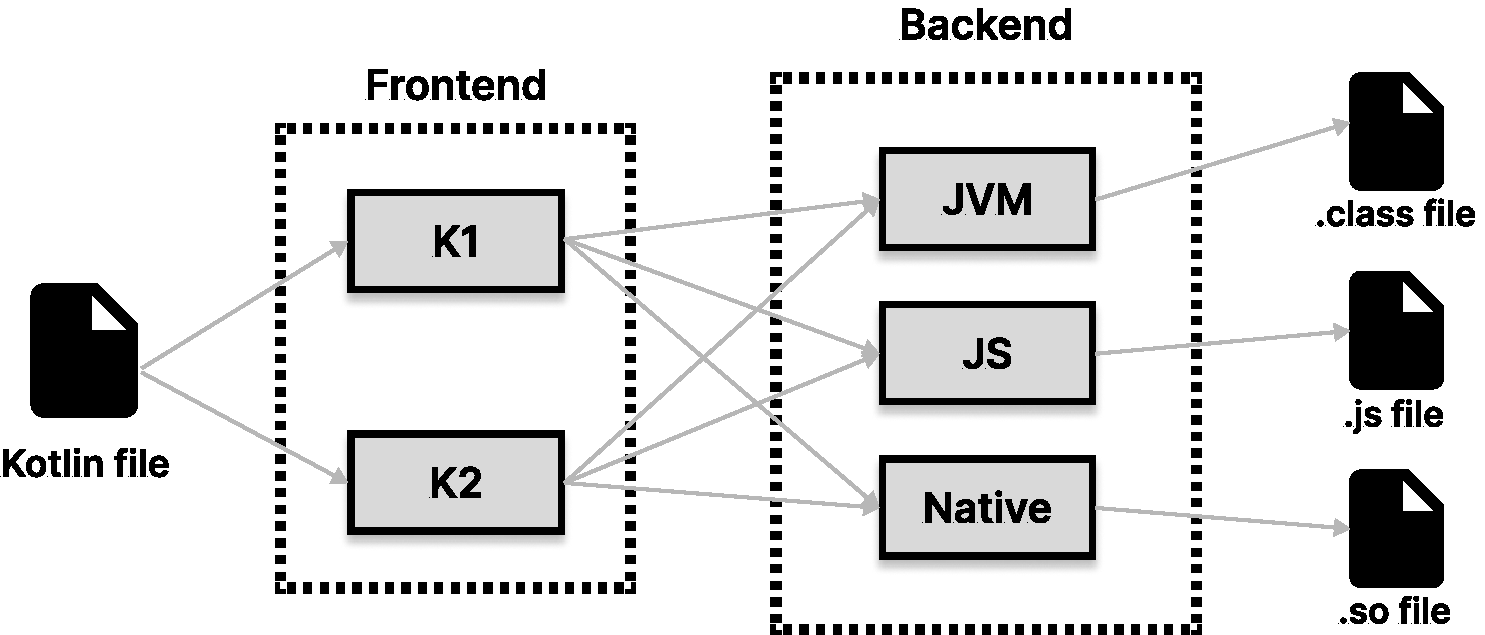
\includegraphics[width=.8\linewidth]{figures/kotlin-compiler-architecture.pdf}
  \caption{Kotlin compiler architecture. Adapted from the one at \cite{moskala2023}}
  \label{fig:kotlin-compiler-architecture}
\end{figure}

The frontend is also responsible for communicating with IDEs and build tools, 
providing APIs to present errors, warnings, code completions and so on. 
%
To make this architecture modular, the Kotlin compiler provides a set of 
\ac{IR}, that the various steps of the workflow
can use to process the preceding steps' output. Both the frontend and the
backend creates this data structure, although they are very different. The 
backend's one is created starting from the output \ac{IR} of the frontend,
while the frontend's one is created from the Kotlin source code. 
The general workflow is summarized in \cref{fig:kotlin-compiler-workflow}.

\begin{figure}
  \centering
  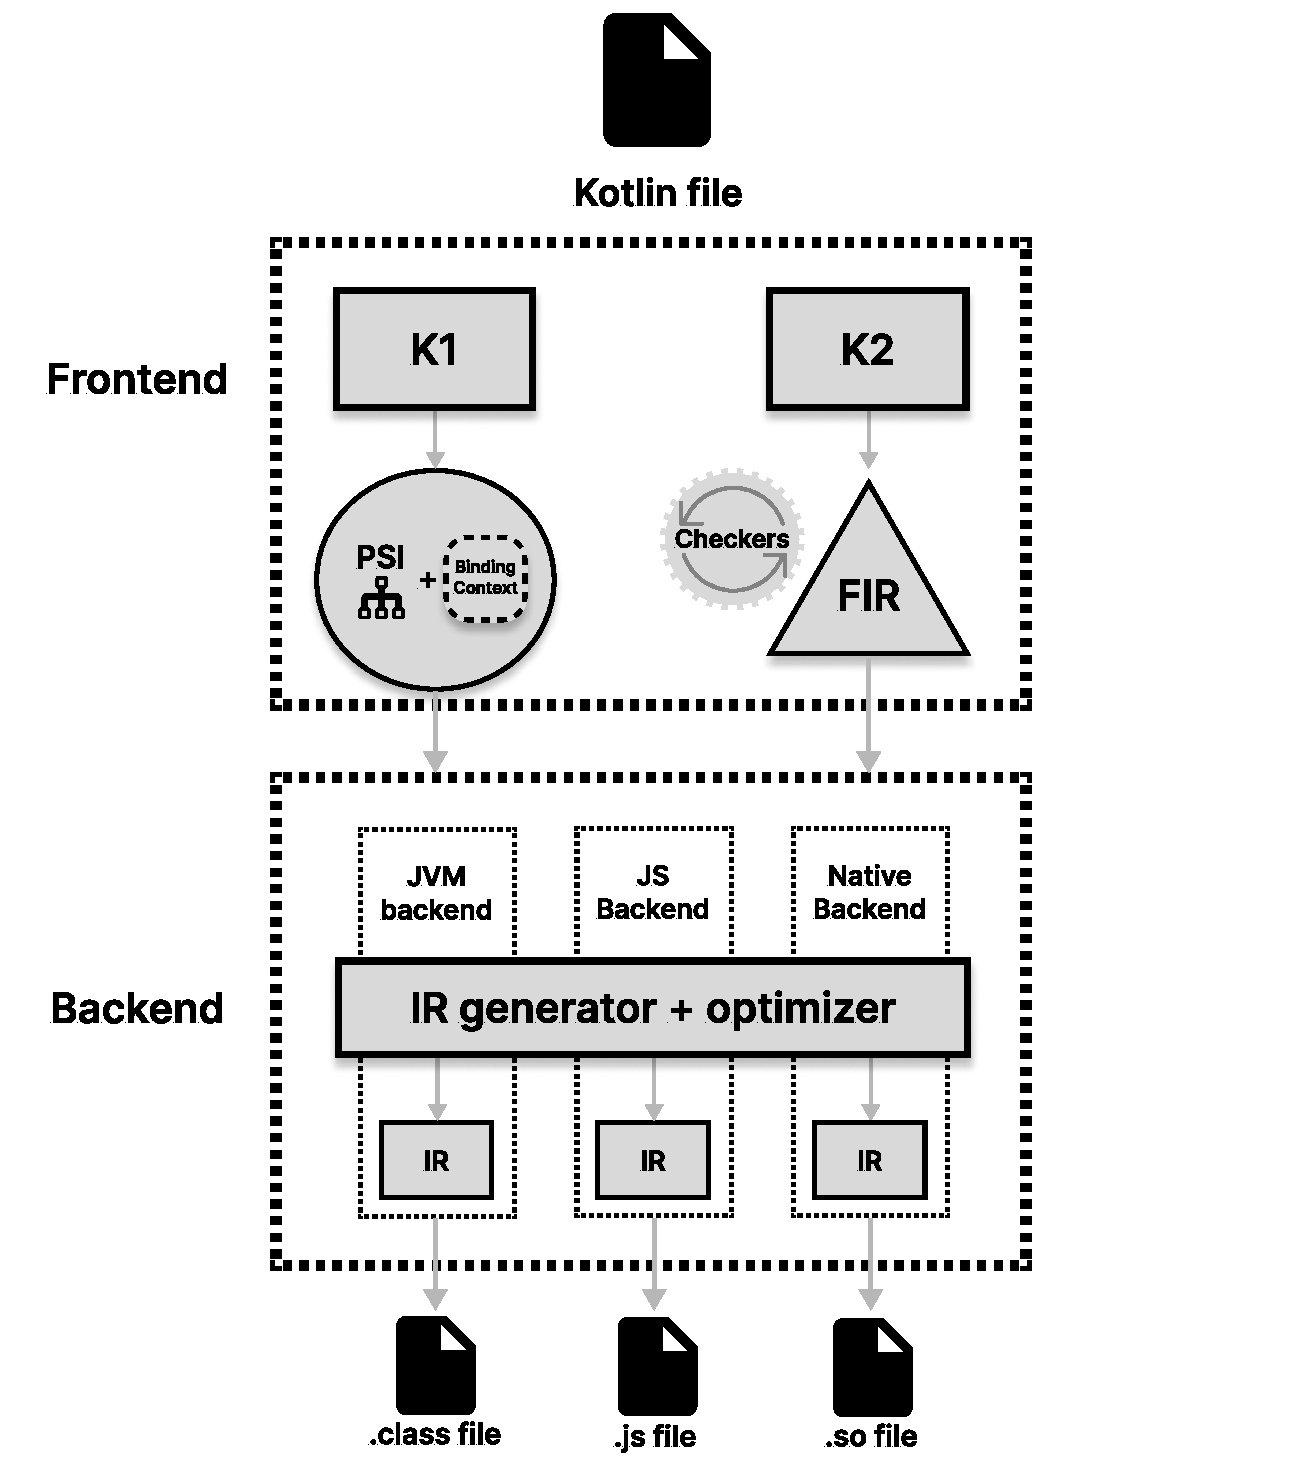
\includegraphics[width=.8\linewidth]{figures/kotlin-compiler-workflow.pdf}
  \caption{Kotlin compiler general workflow. Adapted and extended from the one
  at \cite{moskala2023}}
  \label{fig:kotlin-compiler-workflow}
\end{figure}

Before the so-called K2 frontend the compiler's frontend worked differently,
building the \ac{PSI}, a syntactic model of the parsed source code, and the
\lstinline{BindingContext}, that holds semantic information such as types and
symbol bindings (represented in \cref{fig:kotlin-compiler-workflow} as a whole). 
%
The new K2 frontend, on the other hand, builds the \ac{FIR}, a more powerful and
complete representation of Kotlin parsed code, capable of offloading some of the
work that was previously done by the backend and enabling powerful optimizations
and caching mechanisms. The raw \ac{PSI} is still being produced, but it is now
transformed into the \emph{raw FIR}, which again transforms in different stages,
filling the tree with semantic information. Finally, the resolved tree is passed
to the backend, which takes care of the platform-specific (backend) \ac{IR}, used
to generate the final code.

As we can see in \cref{fig:kotlin-compiler-workflow}, there is still another
process that hasn't been mentioned yet: the \emph{checkers}. During their stage
of execution, the checkers can inspect the \ac{FIR} and reports different
diagnostics. If some of them is considered ``critical'', in the sense that the
compilation should not proceed (e.g., a type error), the compilation is stopped,
and the backend is not executed: otherwise, the final \ac{IR} is passed to it.
%
The role of the checkers is particularly important in the context of this
thesis, and the way it's possible to interact with them is by means of
\textbf{extensions}.

\subsection{Extensions}

Compiler extensions are mechanisms that allow developers to modify various
phases of the compilation process, either by analyzing and transforming code at
the \ac{FIR} level or by modifying the backend \ac{IR}. These extensions
enable advanced features such as additional type checks, automated code
generation, and optimizations, empowering Kotlin’s extensibility.
%
Like with compiler stages, extensions can be either frontend or backend as well.
While frontend extensions impact code analysis, syntax resolution, and IDE
support, backend extensions act right after the \emph{IR generation +
optimization} phase seen in \cref{fig:kotlin-compiler-workflow}. This
distinction makes frontend extensions more suitable for language-level changes
and linting rules, whereas backend extensions are primarily used for performance
optimizations and bytecode transformations.

K2 introduces multiple frontend extensions, all following the
\lstinline{Fir[Name]Extension} convention. In relation to what was previously
discussed, the \lstinline{FirAdditionalCheckersExtension} is particularly
important in this context, since it's a frontend extension that allows
developers to register \emph{additional checkers} to run during compilation.
These checkers can enforce custom coding rules, report warnings, or even prevent
compilation by issuing errors. More over, errors and warnings generated by this
extension appear in IDEs like IntelliJ IDEA, improving real-time code feedback.
This extension is used by Kotlin plugins like \emph{Kotlin Serialization},
which ensures that serialization-related constraints are properly followed, and
\emph{Arrow Meta}, which enforces functional programming best practices.

The extension mechanism is also used in the backend, where backend plugins can
intervene, but the extension that needs to be used in only one:
\lstinline{IrGenerationExtension}. This extension is invoked after the \ac{FIR}
phase has completed and the \ac{IR} has been generated. It allows modifications
to the IR tree before it is used for bytecode generation. Because IR sits
between the frontend and the platform-specific backend, changes made here can
impact the generated machine code without altering the high-level source
representation. 
%
A key limitation of this extension is that it does not influence code analysis
in IntelliJ IDEA. Any method or class injected via this extension will not be
recognized by the IDE, meaning that developers cannot call it directly unless
they use reflection. This extension is widely used in performance-critical
applications. For instance, \emph{Jetpack Compose} leverages it to transform
composable functions into an optimized internal representation. Similarly,
\emph{Kotlin Serialization} uses it to generate serialization methods dynamically,
ensuring they are both efficient and lightweight. However, modifying IR directly
can introduce breaking changes if not handled carefully. Since IR
transformations occur at a low level, even minor alterations can lead to
unintended consequences, making this extension a powerful but complex tool.

Collektive backend plugin uses the \lstinline{IrGenerationExtension} to perform 
the operations we already discussed. To register an extension, the developer needs
to declare a class that extends \lstinline{CompilerPluginRegistrar}. Inside that,
the developer can register the extension using the \lstinline{registerExtension}
method that depends on the type of extension that is being registered. 
%
The core login of the plugin is then implemented in the extension itself. In the
case of the Collektive backend plugin, the class structure is summarized 
in \cref{fig:extensions-class-diagram}.

\begin{figure}
  \centering
  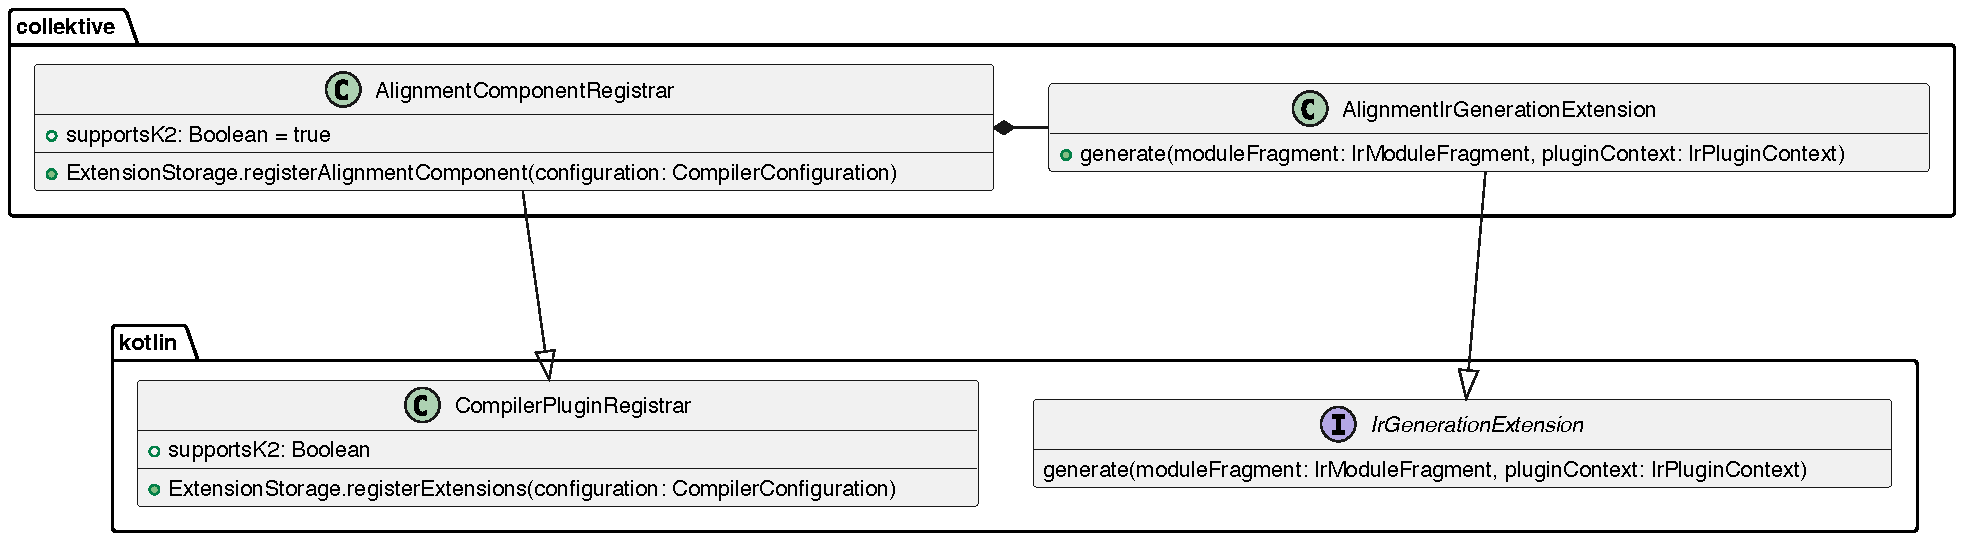
\includegraphics[width=.9\linewidth]{figures/extensions-class-diagram.pdf}
  \caption{Class diagram representing the top-level structure of the Collektive 
  backend compiler plugin. Note: the frontend plugin is not included yet.}
  \label{fig:extensions-class-diagram}
\end{figure}

\section{Motivations}


%----------------------------------------------------------------------------------------
\chapter{Contribution}
\label{chap:contribution}
%----------------------------------------------------------------------------------------

You may also put some code snippet (which is NOT float by default), eg: \cref{lst:random-code}.

\lstinputlisting[float, language=Java, label={lst:random-code}]{listings/HelloWorld.java}

\section{Fancy formulas here}

%----------------------------------------------------------------------------------------
\chapter{Evaluation and Testing}
\label{chap:evaluation}
%----------------------------------------------------------------------------------------

%----------------------------------------------------------------------------------------
\chapter{Conclusion and Future works}
\label{chap:conclusion}
%----------------------------------------------------------------------------------------

%----------------------------------------------------------------------------------------
% BIBLIOGRAPHY
%----------------------------------------------------------------------------------------

\backmatter

\nocite{*} % Remove this as soon as you have the first citation

\bibliographystyle{alpha}
\bibliography{bibliography}

\begin{acknowledgements} % this is optional
Optional. Max 1 page.
\end{acknowledgements}

\end{document}
